\documentclass{exam}
\usepackage{amsmath}
\usepackage{graphicx}
\def\myhrule{\vspace*{0.05in}\lower1ex\null\vadjust{\hrule}}

\pagestyle{head}
\header{\textit{\large Scripps Ranch High Physics Club}}{}{\thepage}
\firstpageheader{\textit{\large Scripps Ranch High Physics Club\myhrule}}{}{\large September 19, 2025 \myhrule}
\begin{document}
    \vspace*{-25px}
    \begin{center}
        \huge \textbf{Lagrangian Mechanics Problem Set}
    \end{center}
    \vspace*{0.05in}
    \Huge
    \begin{center}
        $\frac{\partial L}{\partial q}-\frac{d}{dt}(\frac{\partial L}{\partial \dot{q}})=0$
    \end{center}
    \begin{questions}
        \large
        \question Compute the following partial derivatives
        \begin{parts}
            \part $\frac{\partial}{\partial x} \, y\ln(x^2)-xw^2+e^w$
            \part $\frac{\partial}{\partial y} \, y\ln(x^2)-xw^2+e^w$
            \part $\frac{\partial}{\partial x} \, \cos(xy)+y^2$
            \part $\frac{\partial}{\partial x} \, y\ln(x^2)-xw^2+e^w$
            \part $\frac{\partial}{\partial x} \, y^x+x^y$
            \part $\frac{\partial}{\partial y} \, \cos(\sqrt{x^\pi})-\ln(x!)$
            \part $\frac{\partial}{\partial x} \, \sqrt{x+y}$
        \end{parts}
        \question In Figure 1 we show a box of mass $m$ sliding down a ramp of mass $M$. The ramp moves
without friction on the horizontal plane and is located by coordinate $x_1$. The box also slides without friction
on the ramp and is located by coordinate $x_2$ with respect to the ramp. Find $\ddot{x}_1$
        \begin{center}
            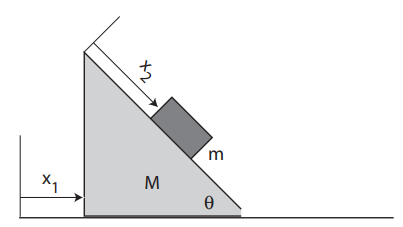
\includegraphics{../assets/figure1.png}\\
            Figure 1
        \end{center}
        \question
    \end{questions}
\end{document}